\chapter{\ac{dis}}

\section{Überblick}
\onehalfspacing
\ac{dis} steht für eine im \ac{ieee} 1278 von 1993 definierten Standard zur Steuerung und Überwachung von Simulationen. Der Standard wird in militärischen sowie in zivilen Simulationen verwendet und  ermöglicht das Erstellen von simmulierten Lagebildern sowie den Datenaustausch der Teilnehmer einer vernetzten Simulation in Echtzeit. Dabei können die Simulationsumgebungen der Teilnehmer unterschiedlich sein.  Um dies zu ermöglichen, wird je eine standardisierte \ac{pdu} für einen Teilnehmer erstellt und an die anderen Teilnehmer im Netzwerk verteilt. Dies ermöglicht die Kommunikation der Teilnehmer.
\\
\ac{dis} wurde in einer Reihe von Workshop des  \ac{ist} der \ac{ucf} entwickelt. Dabei baut \ac{dis} auf den in den 1980er entwickelten \ac{simnet} auf, der für Trainingssimulationen der US Militär geschaffen wurde. Im  Jahr 1996 wurde \ac{hla} entwickelt, dass aus der Verbindung von \ac{dis} und \ac{alsp} besteht.  
\\
Über die Jahre wurde \ac{dis} verbessert und 2012 in der aktuellen Versionen 7 veröffentlicht. Diese Version wurde im \ac{ieee} Standard 1278.1-2012 beschrieben.

\begin{enumerate}
	\singlespacing
	\item \ac{dis} \ac{pdu} Version 1.0  - 1992
	\item \ac{ieee} Standard 1278 - 1993
	\item	\ac{dis} \ac{pdu} Version 2.0 - 1993
	\item 	\ac{dis} \ac{pdu}	Version 2.0 - 1994
	\item 	\ac{ieee} Standard 1278.1 - 1995
	\item 	\ac{ieee} Standard	1278.1a - 1998
	\item 	\ac{ieee} Standard 1278.1 - 2012
		
\end{enumerate}

\cite{SimulationInteroperabilityStandardsOrganizationInc.}
\cite{Wikipedia.31.03.2018}
\cite{MarkMcCall.}
\onehalfspacing
\newpage
\section{Protokoll}
Um die einzelnen Simulationen miteinander zu verbinden, wird eine einheitliche \glqq Sprache\grqq{} benötigt. Die einzelnen Simulationen erstellen \acp{pdu} und broadcasten sie ins Netzwerk, sodass alle anderen Teilnehmer sie empfangen und verarbeiten können. Hierfür wurden in \ac{dis} verschiedene Arten von \acp{pdu} implementiert, die in \ac{pdu}-Familien zusammengefasst wurden. Dabei hat jede \ac{pdu} eine andere Bedeutung und andere Attribute. Im Sinne von \ac{dis} kann eine Entity eine ortsfeste oder ortsveränderliche Einheit darstellen, die spezifische Attribute besitzt. \acp{pdu} enthalten kodierte Informationen, die im \glqq   Enumeration and Bit Encoded Values for Use with Protocols for Distributed Interactive Simulation Applications  \grqq{} enthalten sind. Dabei werden die Informationen nummerisch dargestellt. 
Folgende \ac{pdu}-Familien gibt es:
\begin{itemize}
	\singlespacing
	\item Entity information/interaction
	\item Warfare
	\item Logistics
	\item Simulation Management
	\item Distributed Emission Regeneration
	\item Radio Communications
	\item Entity Management
	\item Minefield
	\item Synthetic Environment
	\item Simulation Management with Reliability
	\item Live Entity
	\item Non-Real Time protocol
	\item Information Operations
	\singlespacing
\end{itemize}

Alle Informationen die eine \ac{pdu} enthalten soll, sind im \ac{ieee} Standard festgelegt. 
Alle \acp{pdu} enhalten einen \ac{pdu} Header, der unter anderem die Protokollversion und den \ac{pdu} Typ enthält.
 Weitere Informationen die der \ac{pdu} Header beinhaltet, sind: 

\begin{itemize}
	\singlespacing
	\item Protocol Version Field					
	 \item Exercise Identifier Field				
     \item 	PDU Type Field					
	\item	Protocol Family Field					
	 \item Time Stamp Field					
	\item PDU Length Field					
	\item Padding Field
\end{itemize}
\onehalfspacing
Im folgenden Absatz wird die Entity information/interaction Familie und die Warfare Familie beschrieben. Diese Familien spielen eine große Rolle innerhalb einer militärischen Simulation.
\\
\subsection{Entity information/interaction }
Die Entity information/interaction Familie besteht aus der  \ac{espdu}, der Entity State Update \ac{pdu} und der Collision \ac{pdu}. Die wichtigste \ac{pdu} ist die  \ac{espdu}, diese enthält Informationen über den Zustand einer Entity, wie zum   Beispiel eine eindeutige Entity ID. Eine weitere wichtige Information ist der Entity Typ, der
 angibt, welcher Nation und Kategorie die Entity angehört.
\\ 
 \begin{table}[H]
 	\centering
 	%\caption{Entity Type Field}
 	\label{Entity_typefield}
 	\begin{tabular}{|l|l|l|}
 		\hline
 		Field size & \multicolumn{2}{l|}{Entity State PDU fields}                        \\ \hline
 		\multicolumn{1}{|c|}{64} & Entity Type & 
 		\begin{tabular}[c]{@{}l@{}}
 			Entity Kind - 8 Bit \\ 
 			Domain - 8 Bit\\ 
 			Country - 16 Bit\\ 
 			Category - 8 Bit\\
 		    Subcategory - 8 Bit \\
 		    Specific - 8 Bit\\
 			Extra - 8 Bit
 	
 
\end{tabular} \\ \hline
  \end{tabular}
\caption{Entity Type Field \cite{SISOStandardsActivityCommitteeoftheIEEEComputerSociety.}} 
\end{table}


\begin{table}[H]
	\centering
	
	\label{entity_examples}
	\begin{tabular}{|l|c|c|c|c|c|c|l|}
		\hline
		& \multicolumn{1}{l|}{Kind} & \multicolumn{1}{l|}{Domain} & \multicolumn{1}{l|}{Country} & \multicolumn{1}{l|}{Category} & \multicolumn{1}{l|}{Subcategory} & \multicolumn{1}{l|}{Specific} & Extra \\ \hline
		Leopard - A6    & 1                         & 1                           & 78                           & 1                             & 3                                & 2                             &       \\ \hline
		M1A2 - Abrams   & 1                         & 1                           & 225                          & 1                             & 1                                & 3                             &       \\ \hline
		T-72B           & 1                         & 1                           & 222                          & 1                             & 2                                & 6                             &       \\ \hline
		Mercedes - C240 & 1                         & 1                           & 78                           & 81                            & 43                               & 3                             &       \\ \hline
		F220 - Hamburg  & 1                         & 3                           & 78                           & 6                             & 3                                & 2                             &       \\ \hline
	
	\end{tabular}
\caption{Entity Type Examples}
\end{table}

Wie in Tabelle \ref{entity_examples} zu sehen ist, bietet die neuste  \glqq Reference for
Enumerations for Simulation Interoperability\grqq{} in der Version 21 \cite{Shanks.} viele verschiedene Beschreibungen für militärische und zivile Einheiten der unterschiedlichsten Länder.

Des Weiteren werden in einer \ac{espdu}  die Geschwindigkeit, die Beschleunigung und die Orientierung angegeben. Der Ursprung der drei Vektoren befindet sich im Massenschwerpunkt. Die Geschwindigkeit und die Beschleunigung setzen sich aus einem  dreidimensionalen Vektor mit den Komponenten X,Y und Z zusammen. Dabei zeigt die X Komponente aus der Vorderseite der Entity. Die Richtung der verbleibenden Komponenten zeigen entsprechend eines rechtwinkligen Koordinatensystems aus der Entity heraus. Der Vektor der die Orientierung angibt, ist in eine Psi ($\psi$), eine Theta ($\theta$)  und eine Phi ($\phi$) Komponente. \\
Neben den genannten Informationen die eine  \ac{espdu} enthält, gibt es noch weitere die im \ac{ieee} Standard beschrieben sind. Diese Informationen sind, wie in Tabelle \ref{Entity_typefield} gezeigt, gegliedert. Jedoch haben sie ihren eigenen Inhalt.
\\
Die Collision \ac{pdu} wird von einer Entity erstellt, wenn diese eine Kollision mit einer anderen Entity oder einem Objekt feststellt. Die Collision \ac{pdu} enthält die Entity IDs der Entity's die zusammenstoßen. Da diese \ac{pdu} im weiteren Verlauf nicht weiter benutzt wird, wird an dieser Stelle davon abgesehen die Collusion \ac{pdu} weiter zu beschreiben. Genaue Informationen können dem \glqq \ac{ieee} Standard 1278.1-2012\grqq{}  \cite{SISOStandardsActivityCommitteeoftheIEEEComputerSociety.} entnommen werden.
\\ 
\cite{MarkMcCall.}
\cite{SISOStandardsActivityCommitteeoftheIEEEComputerSociety.}
\cite{Brann.}
\newpage
\subsection{Entity Warefare}
Die Entity Warefare Familie besteht aus der Fire \ac{pdu}, der Detonation \ac{pdu} , der \ac{de} Fire \ac{pdu} und der Entity Damage Status \ac{pdu}.
Die Fire \ac{pdu} enthält Informationen über das Abfeuern von Waffen, dabei wird unterschieden, ob es sich um eine Waffe handelt oder eine an der Entity angebrachten Verbrauchsmaterial. In \ac{dis} gilt alles als Waffe, das auch als Waffe benutzt werden kann, das kann unter anderem konventionelle Munition, wie beispielsweise Bomben, Raketen, Projektile oder Energiewaffen. Als Verbrauchsmaterial gelten Gegenmaßnahmen gegen Munition wie zum Beispiel IR-Täuschkörpern und sonstiges Verbrauchsmaterial, wie beispielsweise Signalfackeln.  Die Fire \ac{pdu} enthält unter anderem  die Entity ID, der Entity, die gefeuert hat, die beschossen wird, sowie den Abschussort, die verwendete Munition und ob es sich um das Abfeuern einer Waffe oder Verbrauchsmaterial handelt.
Eine Fire \ac{pdu} wird erstellt wenn den Teilnehmern das Abfeuern einer Waffe oder eines Verbrauchsmaterials mitgeteilt werden soll. Sie wird von der Simulation erstellt, die schießt. Sollen andere Entitys die Munition erkennen und eventuell darauf reagieren, muss die Simulation, die die Fire \ac{pdu} erstellt, eine \ac{espdu} erstellen, welche die Munition darstellt. 
\begin{table}[H]
	\centering
	\label{example_munition}
	\begin{tabular}{|l|c|c|c|c|c|c|c|}
		\hline
		& \multicolumn{1}{l|}{Kind} & \multicolumn{1}{l|}{Domain} & \multicolumn{1}{l|}{Country} & \multicolumn{1}{l|}{Category} & \multicolumn{1}{l|}{Subcategory} & \multicolumn{1}{l|}{Specific} & \multicolumn{1}{l|}{Extra} \\ \hline
		AIM-9B Sidewinder & 2                         & 1                           & 225                          & 1                             & 1                                & 1                             &                            \\ \hline
		Tomahawk          & 2                         & 10                          & 225                          & 1                             & 4                                &                               &                            \\ \hline
		5.56 mm           & 2                         & 8                           & 78                           & 2                             & 1                                &                               &                            \\ \hline
		120 mm HE         & 2                         & 9                           & 78                           & 2                             & 5                                & 1                             &                            \\ \hline
	\end{tabular}
	\caption{Beispiel Munition}
\end{table}

Da Raketen, wie die AIM-9B Sidewinder, Marschflugkörper, wie die Tomahawk,   klassische Projektile wie die 5,56 mm Munition, für Sturmgewehre oder 120mm HE Geschosse, für zum Beispiel Panzer, als Munition gelten, können diese durch eine  \ac{espdu} mit den entsprechenden Attributen repräsentiert werden. 
\\
Die Detonation \ac{pdu} enthält, ähnlich wie die Fire \ac{pdu},  die Entity ID der Entity, die gefeuert hat und die, die beschossen wird. Es ist neben anderen Informationen auch der Ort der Detonation, sowie die Entity ID der Munition bzw. des Verbrauchsmaterials, welches abgefeuert wurde, enthalten. Eine Detonation \ac{pdu} wird erstellt, wenn der Einschlag oder die Explosion einer  Munition, das Umsetzen von Verbrauchsmaterial  oder sonstigen Explosionen den Teilnehmern mitgeteilt werden soll. 
Bei der Detonation\ac{pdu} kommt neben der Munitions ID ein sogenannter \glqq Burst Descriptor Record \grqq zur Verwendung. Dieser enthält neben der Munition auch die Angaben des verwendeten Sprengkopfs, des Zünders, die Anzahl der Schüsse und die Feuerrate.
Soll die Entity, bei der die Munition einschlägt und detoniert, als zerstört gelten, muss die  \ac{espdu} deaktiviert werden. Wird die Entity nicht zerstört, kann der  \ac{espdu} ein Schaden zugewiesen werden. Entstehen bei der Detonation Fragmente der ursprünglichen Entity, können diese Fragmente ebenfalls als  \acp{espdu} dargestellt werden.
\\
\cite{MarkMcCall.}
\cite{SISOStandardsActivityCommitteeoftheIEEEComputerSociety.}
\cite{Brann.}
\cite{JDBEatFt.HuachucaArizona.13.10.2003}
\subsection{Koordinaten System}
Das Koordinatensystem, nach dem  in \ac{dis} Positionsangaben getätigt werden, ist das \ac{wgs}.
\ac{wgs} ist ein in den 1980ern entwickeltes geodätisches Referenzsystem zur Standardisierung von Positionsangaben auf der Erde und im erdnahen Weltraum.
\ac{wgs} besteht aus mehreren Bestandteilen. Es beinhaltet einen Referenzellipsoiden, welcher der stark vereinfachten Oberfläche der Erde angepasst wurde und für Ortsangaben in Form von geografischer Länge und Breite genutzt wird. Des Weiteren beinhaltet \ac{wgs} einen detailliertes Modell der Erde, welches stark von dem Referenzellipsoiden abweicht. Dieses Modell wird als Geoid bezeichnet. 
\begin{figure}[H]
	\centering
	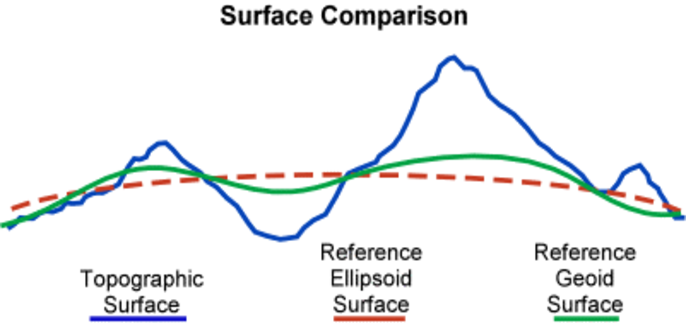
\includegraphics[width=0.7\textwidth]{bilder/surfacecomparison.pdf}
	\caption{Unterschied Geoid, Ellisoid und realer Oberfläche \cite{UNAVCO.22.03.2018}}
	\label{img:oberflächenunterschied}
\end{figure}
Als dritte Komponente beinhaltet \ac{wgs} eine dreidimensionales Koordinatensystem.
Wie man in der Abbildung \ref{img:wgs84} sehen kann, handelt es sich hierbei um kartesisches Koordinatensystem, welches seinen Ursprung im Erdmittelpunkt hat. Die Orientierung des Koordinatensystems wurde durch das \ac{bih} vorgegeben. Die Z-Achse geht vom Ursprung aus durch den Nordpol des Ellipsoiden. Sie dient dabei als Rotationsachse. Die X-Achse verläuft vom Ursprung aus durch den Nullmeridian auf der Höhe des Äquators. Dabei steht sie senkrecht zur Z-Achse. Die Y-Achse verläuft senkrecht zu den beiden anderen Achsen auf der Höhe des Äquators und komplettiert das kartesische Koordinaten System. 

\begin{figure}[H]
	\centering
	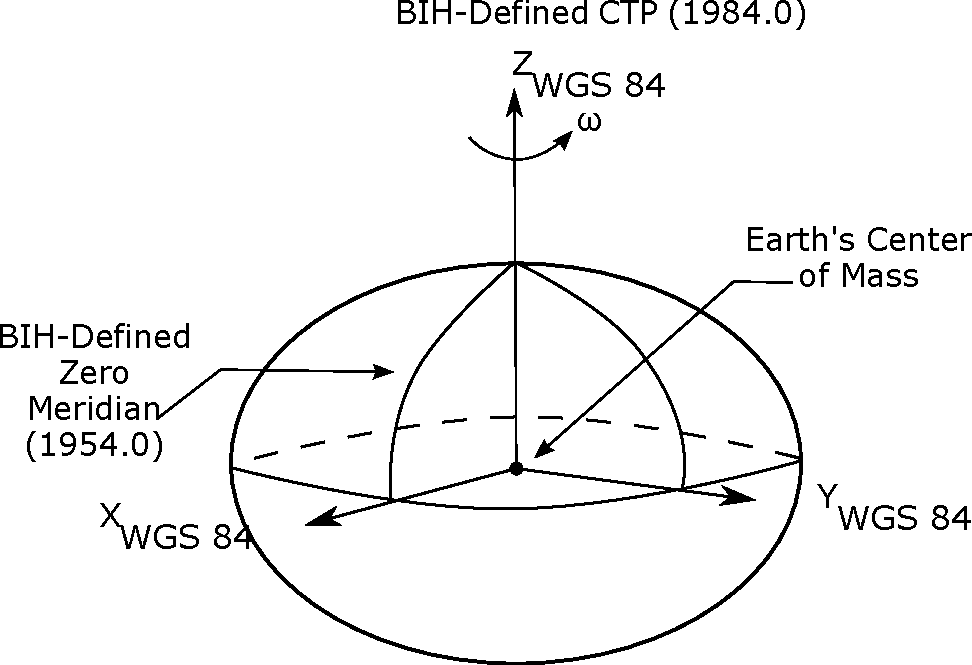
\includegraphics[scale=0.5]{bilder/wgs84.pdf}
	\caption{WGS 84 \cite{DefenseMappingAgency.}}
	\label{img:wgs84}
\end{figure}
\ac{dis} nutzt das die dreidimensionale Angabe von Koordinaten als globales Koordinatensystem. Dies ermöglicht die genaue Positionierung von Entitys. Zusätzlich zu dem globalen Koordinatensystem hat jede Entity noch ihr eigenes lokales Koordinatensystem. Dieses besteht auch aus einem kartesischen Koordinatensystem mit den Komponenten X,Y und Z. Die Komponenten haben als gemeinsamen Ursprung den idealisierten Massenschwerpunkt der Entity.  
Die X Koordinate zeigt dabei aus der Front der Entity heraus. Die Y Koordinate zeigt im rechten Winkel zur X Achse an der rechten Seite der Entity heraus. Die Z Achse zeigt vom Ursprung nach unten. Die Größenordnung des Koordinatensystems ist wie beim \ac{wgs} in Metern. 
\begin{figure}[H]
	\centering
	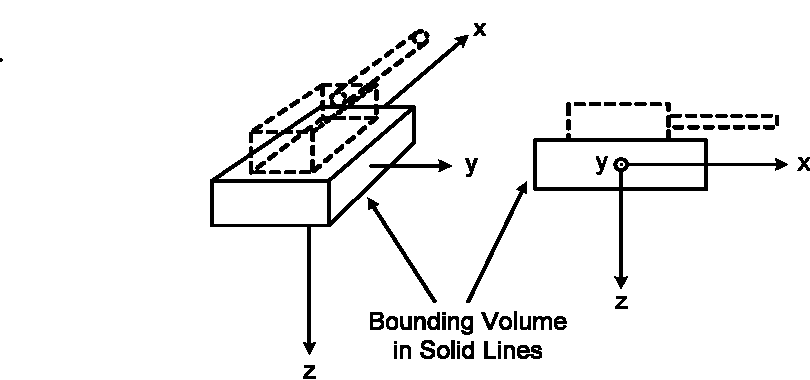
\includegraphics[scale=0.7]{bilder/entity_koordinaten.pdf}
	\caption{Entity Koordinatensystem \cite{SISOStandardsActivityCommitteeoftheIEEEComputerSociety.}}
	\label{img:wgs84}
\end{figure}

\section{Anforderungen}
Das \ac{dis} Protokoll ist ein Mittel um verschiedene Simulationen mit einander zu verbinden. Jedoch müssen dafür einige Anforderungen eingehalten werden. Eine \ac{dis} Übung, also eine Verknüpfung von Simulationen, muss mindestens zwei Simulationen enthalten, die mit einander vernetzt sind. Sollen die vernetzten Simulationen Ereignisse oder Aktivitäten auslösen, ist das \ac{dis} Protokoll zu verwenden.  Auch hierbei werden verschiedene Anforderungen gestellt. Um festzulegen, welche Simulationen an einer Übung teilnehmen, wird eine eindeutige Übungs-ID an die Simulationen verteilt, die an dieser teilnehmen. Jede Simulation muss durch ein \glqq Simulation Address record\grqq{} identifiziert werden. Dieser Record ist im \ac{ieee} Standard festgelegt und enthält die \glqq Site Number\grqq{} und die  \glqq Application Number\grqq{}.
Die \glqq Site Number\grqq{} und die \glqq Application Number\grqq{} stellen die Zugehörigkeit zu einer Übung dar, dabei dürfen zwei unterschiedliche Simulationen nicht den selben \glqq Simulation Address record\grqq{} haben.  
Stellt eine Simulation eine Entity dar, muss eine Entity ID zugewiesen werden, mit der \acp{pdu} ausgegeben werden können die sich auf diese Spezielle Entity beziehen. Hier wird die \glqq Site Number\grqq{} und die  \glqq Application Number\grqq{} im Header angegeben. Werden  mehrere Entitys in einer Simulation erstellt, sind die  \glqq Site Number\grqq{} und die   \glqq Application Number\grqq{} gleich.
Als weitere Anforderung gilt, dass alle Teilnehmer einer Simulation von einander wissen müssen. Das bedeutet, dass die Informationen über Entitys oder Ereignisse an alle Teilnehmer verteilt werden müssen, dies lässt sich als Broadcast realisieren. 
\chapter{Beispielsimmulation}
Im folgenden Kapitel wird eine Beispiel Simulation beschrieben, die auf dem \ac{dis}-Protokoll beruht. Dabei wird eine \ac{dis} Library verwendet, die auf dem Standard \ac{ieee}-1278.1 beruht.
Hierbei wird eine \glqq open source\grqq{} Implementation mit dem Namen \glqq Open-DIS\grqq{} verwendet, die vom \ac{moves}-Institute an der Naval Postgraduate School der US Navy in Monterey (Kalifornien) entwickelt wurde.   \glqq Open-DIS\grqq{} wurde in verschiedenen Sprachen implementiert. Dazu zählen Java, JavaScript, C++, Python und CSharp. Die im Rahmen dieser Arbeit verwendete Implementation wurde in der Programmiersprache C++ geschrieben.    Diese Library enthält eine grundlegende Version von \ac{dis}. Dazu gehören die verschiedensten \acp{pdu}, mathematische Gebilde, die benötigt werden und Funktionen, mit denen \acp{pdu} Attribute und Eigenschaften hinzugefügt werden können. \cite{.13.10.2017}

\section{Ziel der Beispielsimulation}
Das Ziel der  Simulation war es, erste Erfahrungen mit der Library zu machen und die Möglichkeiten abzugrenzen, die \glqq open source\grqq{} bietet. Des Weiteren sollte eine Einschätzung getroffen werden, ob \glqq open source\grqq{} in Verbindung mit anderen Bibliotheken eine Plattform liefert, auf der Simulationen einfach zu realisieren sind.

\section{Beispiel einer \ac{espdu}} 
Um diese Fragen zu beantworten, wurde ein fiktives Szenario erstellt, in dem zwei Landeinheiten enthalten sind, die sich bewegen und  schießen beziehungsweise explodieren können. 
Zu Beginn einer Simulation wird ein Zwischenspeicher benötigt, der dem \ac{dis} Format entspricht. In diesem Speicher werden die zu versendenden Daten gespeichert.   
Anschließend kann die erste \ac{espdu} erstellt werden. In Quellcode \ref{lst:unitheader} ist zu sehen, wie eine \ac{espdu} erstellt wurde. Ihr wurde eine Protokollversion, eine ExerciseID, sowie die in der Entity ID enthaltenen Site, Application und Entity Nummer gegeben. Dabei muss die Entity ID erst als eigenständiges Feld erstellt und befüllt werden, bevor man einer \ac{espdu} eine Entity ID geben kann.

\begin{lstlisting}[caption=Unit Header,label={lst:unitheader}]
DIS::EntityStatePdu unit1;
unit1.setProtocolVersion(6);
unit1.setExerciseID(0);
  
DIS::EntityID unit1_entity_id;
	unit1_entity_id.setSite( 0 );
	unit1_entity_id.setApplication( 1 );
	unit1_entity_id.setEntity( 1 );
  
unit1.setEntityID(unit1_entity_id);
  
\end{lstlisting}
Im Quellcode \ref{lst:entity_typ} wird dem Entity Typ, wie in Tabelle \ref{entity_examples} zu sehen, bestimmte Attribute zugewiesen. In diesem Fall handelt es sich um einen Leopard 2 A6.
Das Zuweisen des Typs erfolgt, wie bei der Entity ID, erst nach dem Erstellen des Typs. 
\begin{lstlisting}[caption=Entity Typ,label={lst:entity_typ}]
DIS::EntityType leo2;
	leo2.setCategory( 1 );
	leo2.setCountry( 78 );
	leo2.setDomain( 1 );
	leo2.setEntityKind( 1 );
	leo2.setExtra( 0 );
	leo2.setSpecific( 2 );
	leo2.setSubcategory( 3 );

unit1.setEntityType( leo2 );
\end{lstlisting}
Neben den grundsätzlichen Informationen, die man einer Entity geben kann, können auch Informationen über zusätzliche Teile hinzugefügt werden. Diese Teile können beweglich oder fest angebracht sein. 
In dem Beispiel  \ref{lst:att_parts} wird dem  Panzer ein Turm und eine Hauptkanone hinzugefügt. Dabei wird durch einen zusätzlichen Parameter dem Turm eine Drehgeschwindigkeit gegeben. Die Hauptkanone, also das Rohr, hat keine entsprechende Neigungsgeschwindigkeit, da diese Geschwindigkeit so groß ist, das sie keinen entsprechenden Einfluss hat.
Jedes Teil, das hinzugefügt werden soll, ist vom Grundaufbau gleich. Über den Wert \glqq ParameterType \grqq{} kann die Art des Teils festgelegt werden. Alle möglichen Teile können  der \glqq Enumeration\grqq{} entnommen werden. Über den Wert \glqq{}  PartAttachedTo\grqq{} kann festgelegt werden, wo das Zusatzteil angebracht ist. Eine \glqq 0\grqq{} gibt an, dass es direkt mit der Entity verbunden ist. Ein anderer Wert steht für den Index eines anderen Teils, an dem das zu spezifizierende Zusatzteil befestigt ist. Der  \glqq ParameterTypeDesignator\grqq{} gibt an, ob es sich um ein starres oder ein bewegliches Teil handelt. Um zum Beispiel der Kanone  eine Neigung zu geben, wird die entsprechende Gradzahl im  \glqq ParameterValue\grqq{} angegeben.
Alle Teile, dem man an der Entity anbringen will, werden erst in einen Vektor geschrieben, der dann der \ac{espdu}  angehängt wird.
 
 \begin{lstlisting}[caption=Zusatz Teile,label={lst:att_parts}]
  ArticulationParameter turret_azimuth;
 turret_azimuth.setParameterType( 4096 );
 turret_azimuth.setPartAttachedTo( 0 );
 turret_azimuth.setParameterTypeDesignator( 0 );
 turret_azimuth.setParameterValue(0*PI/180);
 
 ArticulationParameter turret_azimuth_rate;
 turret_azimuth_rate.setParameterType( 4096 );
 turret_azimuth_rate.setPartAttachedTo( 0 );       
 turret_azimuth_rate.setParameterTypeDesignator( 0 );
 turret_azimuth_rate.setParameterValue( 0 );
 
  ArticulationParameter turret_gun_elevation;
 turret_gun_elevation.setParameterType( 4416 );
 turret_gun_elevation.setPartAttachedTo( 1 );            
 turret_gun_elevation.setParameterTypeDesignator( 0 );
 turret_gun_elevation.setParameterValue( 0 );

 
 
 std::vector<DIS::ArticulationParameter> params;
 params.clear();
 params.resize(3);  // make default number of parameters
 params[0] = turret_azimuth;
 params[1] = turret_azimuth_rate;
 params[2] = turret_gun_elevation;
 
 
 unit1.setArticulationParameters(params);
 
 
 
 
 \end{lstlisting}
 
 
Um nun der \ac{espdu} einen Standort zu geben, wird auf die gleiche Weise verfahren. Erst muss man einen Standort erstellen, dem man der \ac{espdu} dann anschließend zuweisen kann. Wie ein Standort genau erstellt wird und welche Probleme dabei aufgetreten sind, wird in  \ref{gelös_probl} erklärt. Wenn man nun die Entity in eine bestimmte Richtung bewegen will, wird zunächst ein Beschleunigungsvektor benötigt, der dann über eine Funktion der Entity hinzugefügt wird. Auf gleiche Weise wird auch die Orientierung der Entity hinzugefügt. In Quellcode \ref{lst:velo_hedding} ist zu sehen, wie der Entity eine Geschwindigkeit von 1m/s, in X - Richtung und einer Richtung von 180°, vom eigenen Standpunkt aus gegeben wird.

\begin{lstlisting}[caption = Beschleunigungs- und Orientierungsvektor,label={lst:velo_hedding}]
DIS::Vector3Float veloUnit1;
	veloUnit1.setX(1);
	veloUnit1.setY(0);
	veloUnit1.setZ(0);

DIS::Orientation headding_unit1;
	headding_unit1.setTheta(0);
	headding_unit1.setPsi(180);
	headding_unit1.setPhi(0);

unit1.setEntityOrientation(headding_unit1);
unit1.setEntityLinearVelocity(veloUnit1);
\end{lstlisting}

Um  diese \ac{espdu} über ein Netzwerk zu senden, müssen die Daten noch serialisiert werden.   
\begin{lstlisting}[caption = Serialisieren der Entity,label={lst:marshal}]
DIS::DataStream buffer( DIS::BIG );

unit1.marshal(buffer);
/*code for sending buffer */
\end{lstlisting}
\newpage
\section{Gelöste Probleme}\label{gelös_probl}
Während die Beispielsimulation erstellt wurde, traten größere und kleinere Probleme auf. In diesem Abschnitt werden nur die größten gelösten Probleme beschrieben. Im Abschnitt \ref{open_prob} werden die nicht gelösten Probleme beschrieben.\\
Das größte Problem das auftrat, war das der Positionsberechnung. Da \ac{dis} als Koordinatensystem das \ac{wgs} benutzt musste zunächst eine Möglichkeit gefunden werden \ac{gps} Koordinaten, die In Breite- und Längengrad angegeben sind, in einen dreidimensionalen Vektor umzurechnen.
Eine mögliche Lösung dafür bietet die \glqq GeographicLib\grqq{}.
Die \glqq GeographicLib\grqq{} bietet nicht nur eine Lösung für das Umrechnen von Koordinaten, mit ihrer Hilfe lassen sich auch der Abstand und die Richtung von Koordinaten berechnen. Des Weiteren kann man mit der Library Punke um eine bestimmte Entfernung in eine bestimmte Richtung versetzen. Diese Funktion ermöglicht eine Konstante Positionsänderung, also das Berechnen der Bewegung einer Entity. \\
Um Funktionen der \glqq GeographicLib\grqq{} zu nutzen, muss man zunächst die Referenz-ellipsoiden und den Referenz-geoid erstellen. 
Dies ist durch einen Funktionsaufruf, wie im Codebeispiel \ref{lst:ref} zusehen, möglich.

\begin{lstlisting}[caption = Referenz-Ellipsoid und Geoid ,label={lst:ref}]
Geocentric earth(Constants::WGS84_a(), Constants::WGS84_f());
Geodesic geod(Constants::WGS84_a(), Constants::WGS84_f());
\end{lstlisting}
Im Beispiel \ref{lst:calc} sieht man den Aufruf der Funktion die von einer \ac{gps} Koordinate in eine geozentrische Koordinate umrechnet und der Funktion die wieder zurückrechnet.
Als Input benötigen die Funktionen jeweils das Quellsystem und das Zielsystem in das Umgerechnet werden soll. \\
\begin{lstlisting}[caption = Umrechnung der Koordinaten ,label={lst:calc}]
// from GPS to XYZ 
earth.Forward(Latitude,Longitude,Height_above_geoid,X,Y,Z);

//from XYZ to GPS
earth.Reverse(X,Y,Z,Latitude,Longitude,Height_above_geoid);
\end{lstlisting}
In \ref{lst:geod_calc} wird gezeigt, wie Berechnungen innerhalb eines Koordinatensystems durchgeführt werden. Im als erstes wird eine Position berechnet die in einer bestimmten Entfernung und Richtung ausgehend von einer Startposition liegt. Die zweite Funktion berechnet den Abstand und die Richtungen der beiden Positionen zueinander.  
\begin{lstlisting}[caption = Berechnungen innerhalb eines Systems ,label={lst:geod_calc}]
//move from position A to a new position
geod.Direct(Latitude,Longitude,Direction,Length,
            Latitude_new,Longitude_new);

//distance and direction from position A to position B
geod.Inverse(Latitude0,Longitude0,Latitude1,Longitude1,
	     Length,Direction0,Direction1);

\end{lstlisting}

Alle dargestellten Beispielfunktionen der \glqq GeographicLib\grqq{} gehören zu  Klassen von Funktionen die in der Dokumentation der Library ausführlicher erklärt werden.
\\
Da für das Senden und Empfangen von \ac{dis} Paketen  \ac{udp}  verwendet wird ist stellt das versenden der Pakete nicht das Problem dar, jedoch war das verarbeiten von empfangen Paketen ein Problem. Da der Client, der ein Paket in \ac{dis} Format bekommt, nicht weiß um was es sich bei diesem Paket handelt, musst eine Möglichkeit gefunden werden dies heraus zu finden. Das Extrahieren der Klasse stellte im Großen und Ganzen nicht das Problem dar, denn im Header einer \ac{pdu} steht, um was es sich bei dieser \ac{pdu} handelt. Jedoch musst diese Grundlegende-\ac{pdu} noch in die entsprechende \ac{espdu}, Fire \ac{pdu}, Detonation \ac{pdu} oder in eine Andere umgewandelt werden. Um aus den empfangenen Daten eine \ac{pdu} zu machen, muss eine \glqq\ac{pdu}-Factory\grqq{} verwendet werden.  
Diese erstellt aus den empfangen Daten, die als ein Vektor vorliegen, eine \ac{pdu}. \\
\\
\begin{lstlisting}[caption = PDU Factory ,label={lst:factory}]
DIS::PduFactory pf;

DIS::Pdu *recvPDU;
recvPDU = pf.createPdu(DATASTREAM);
\end{lstlisting}
Da der Empfänger nicht weiß, wie viele \acp{pdu} er bekommt, wurde als Zwischenspeicher eine \glqq map\grqq{}  verwendet. In der \glqq map\grqq{} wird die \ac{pdu} mit der Hilfe eines KEYs gespeichert. Dieser Key setzt sich aus der Entity ID zusammen. Im Codebeispiel \ref{lst:factory} ist gezeigt, wie durch das Abfragen des \ac{pdu} Typs eine Entsprechende \ac{pdu} erstellt wird. Das dargestellte Beispiel ist nicht vollständig, jedoch sind die anderen Cases in ähnlicher weise Aufgebaut.

\begin{lstlisting}[caption = PDU-Typ kovertieren ,label={lst:factory}]
std::map<int,DIS::EntityStatePdu> unitmap;

int pdutype = (int)(*recvPDU).getPduType();

switch (pdutype) {
case 0x1:
	EntityStatePdu *helppdu;
	helppdu = (DIS::EntityStatePdu *)pf.createPdu(help);
	key = keymaker((*helppdu).getEntityID());
	unitmap[key] = *helppdu;
break;
.
.
.
\end{lstlisting}
       
Neben den genannten gelösten Problemen, traten noch weitere kleine Probleme auf die jedoch keine speziellen Lösungen erstellt wurden.
\section{Offene Probleme}\label{open_prob}
Im laufe der Erstellung der Beispielsimulation traten auch Probleme auf, für noch keine, oder keine zufriedenstellende Lösung gefunden wurde. Eines dieser Probleme ist die Darstellung der Entitys auf einer Karte.   

\section{Fähigkeiten der Beispielsimulation}

\section{Ausblick}
\chapter{Fazit}